
\chapter{Los datos: origen, descripción y análisis}
\label{cap:datos}

\section{Introducción}
\label{sec:introduccion_datos}
En este capítulo se detalla el conjunto de datos utilizado para el desarrollo e integración del sistema de Inteligencia Artificial del proyecto \textit{Cupid Algorithm}. A diferencia de los problemas de clasificación tradicional, donde se perfila a un individuo de forma aislada, el presente reto analítico requiere el estudio de una \textbf{diada} (la pareja concebida como unidad matemática). 

El objetivo principal de esta sección es comprender cómo interactúan y se correlacionan los perfiles psicológicos y demográficos, establecer las métricas formales de éxito y definir los procesos de transformación de datos (\textit{Feature Engineering}) necesarios para alimentar el modelo predictivo. Durante el desarrollo del análisis se abordará el debate psicológico subyacente sobre si la afinidad relacional se fundamenta en la complementariedad (polos opuestos) o en la homofilia (similitud), justificando empíricamente las decisiones algorítmicas adoptadas.

\section{Fuentes, origen y tamaño de los datos}
\label{sec:fuentes_datos}
La fuente de información para realizar esta investigación es \texttt{cupid\_algorithm\_dataset.csv}. Este \textit{dataset} emula el entorno operativo de una aplicación de emparejamiento (\textit{matchmaking}) a gran escala, registrando interacciones reales entre usuarios.

En términos de volumetría, la muestra consta de \textbf{100.000 observaciones} (pares evaluados) y 30 características originales. La magnitud y completitud del conjunto de datos garantizan la representatividad estadística necesaria para entrenar modelos de aprendizaje automático de alta complejidad, mitigando el riesgo de sobreajuste (\textit{overfitting}) temprano. Asimismo, la validación de calidad del dato evidenció una estructura robusta: la inspección inicial confirmó la ausencia total de valores nulos o faltantes, lo cual permite prescindir de técnicas de imputación sintética que pudieran introducir sesgos artificiales en las distribuciones originales.

\section{Inventario de datos}
\label{sec:inventario_datos}
La base de datos presenta una arquitectura simétrica, registrando idéntica batería de atributos tanto para el ``Individuo A'' como para el ``Individuo B'' de cada emparejamiento. Estas variables se agrupan formalmente en las siguientes dimensiones:

\begin{itemize}
    \item \textbf{Dimensión Demográfica y Sociológica:} Contiene atributos descriptivos tales como la edad, el nivel educativo (modelado como variable ordinal), la ubicación geográfica o entorno de residencia (\texttt{location}) y el campo profesional o sector productivo al que pertenecen (\texttt{career\_field}).
    
    \item \textbf{Dimensión Psicológica y Conductual:} Agrupa valores normalizados en el rango [0, 1] que cuantifican la ambición profesional, la expresividad emocional, la espontaneidad y el cronotipo de cada sujeto. Resulta especialmente relevante la inclusión del modelo de los Cinco Grandes (\textit{Big Five}): apertura a la experiencia (\texttt{openness}), extraversión, amabilidad (\texttt{agreeableness}) y responsabilidad (\texttt{conscientiousness}). Adicionalmente, se tipifica el estilo afectivo de los individuos mediante su lenguaje del amor principal.
    
    \item \textbf{Variables Objetivo (\textit{Targets}):} Representan la verdad terreno (\textit{ground truth}) con la que se evaluará el desempeño del sistema:
    \begin{itemize}
        \item \texttt{compatibility\_score}: Puntuación continua que evalúa la calidad y viabilidad general del emparejamiento (problema de regresión).
        \item \texttt{compatible}: Etiqueta binaria de clasificación donde se codifica el éxito (1) o el fracaso (0) de la relación.
        \item \texttt{relationship\_longevity\_months}: Duración efectiva de la relación expresada en meses.
    \end{itemize}
\end{itemize}

Para facilitar la comprensión global de la estructura base del sistema, la Tabla~\ref{tab:inventario_datos} detalla el diccionario de datos original. Se listan las variables de manera genérica, asumiendo que el modelo procesa las características tanto del individuo A (\texttt{a\_*}) como del individuo B (\texttt{b\_*}).

\begin{table}[H]
\centering
\footnotesize % <-- Comando añadido para reducir el tamaño de la fuente de la tabla
\begin{tabular}{llp{10.5cm}}
\hline
\textbf{Variable} & \textbf{Tipo} & \textbf{Descripción} \\ \hline
\texttt{pair\_id} & Entero & Identificador único (1 a 100,000) de cada pareja evaluada. Actúa como clave primaria. \\
\texttt{age} & Numérica & Edad cronológica (18-55). Se emplea para calcular la brecha de edad; diferencias superiores a 15 años penalizan el \textit{score}. \\
\texttt{education} & Ordinal & Nivel educativo (1: Secundaria - 5: Doctorado). Correlaciona positivamente con la ambición profesional. \\
\texttt{location} & Categórica & Entorno de residencia (Urbano, Suburbano, Rural). Las coincidencias suman positivamente al evaluar la proximidad. \\
\texttt{career\_field} & Categórica & Sector profesional (10 industrias). Su compatibilidad cruzada se evalúa internamente mediante una matriz de sinergia. \\
\texttt{career\_ambition} & Num. [0,1] & Impulso de crecimiento profesional. La proximidad de valores entre la pareja indica alineación de proyectos de vida. \\
\texttt{openness} & Num. [0,1] & Rasgo \textit{Big Five}: apertura a la experiencia, ideas nuevas y creatividad. \\
\texttt{extraversion} & Num. [0,1] & Rasgo \textit{Big Five}: nivel de extroversión, sociabilidad, energía y asertividad social. \\
\texttt{agreeableness} & Num. [0,1] & Rasgo \textit{Big Five}: amabilidad, tendencia a la compasión, empatía y voluntad de compromiso. \\
\texttt{conscientiousness} & Num. [0,1] & Rasgo \textit{Big Five}: nivel de organización, disciplina y responsabilidad personal. \\
\texttt{chronotype} & Num. [0,1] & Preferencia de estilo de vida que abarca desde perfiles nocturnos hasta matutinos. \\
\texttt{spontaneity} & Num. [0,1] & Orientación vital entre la planificación estructurada (0) y el espíritu libre (1). \\
\texttt{emotional\_express...} & Num. [0,1] & Estilo de comunicación: facilidad y franqueza al expresar y compartir sentimientos íntimos. \\
\texttt{love\_language} & Categórica & Lenguaje del amor principal (Palabras de afirmación, Actos de servicio, Regalos, Tiempo de calidad o Contacto físico). \\
\texttt{compatibility\_score}& Continua & \textbf{Target:} Puntuación predictiva agregada (0-100) que determina la compatibilidad base de la pareja. \\
\texttt{compatible} & Binaria & \textbf{Target:} Éxito relacional (1) o fracaso (0). Umbral original establecido en >65 de \textit{score}. \\
\texttt{relationship\_lon...} & Entero & \textbf{Target:} Longevidad de la relación expresada en meses (0-120). Útil para problemas de regresión o supervivencia. \\ \hline
\end{tabular}
\caption{Inventario de datos original: Diccionario de variables}
\label{tab:inventario_datos}
\end{table}

Para ilustrar de forma tangible esta arquitectura simétrica, las Figuras~\ref{fig:registros_a} y~\ref{fig:registros_b} muestran, de manera independiente, los perfiles de los usuarios vinculados que conforman los primeros 24 registros del conjunto de datos. Como se puede observar, ambos sujetos (Individuo A e Individuo B) mantienen de forma estricta el mismo identificador de pareja (\texttt{pair\_id}). Esta restricción relacional es la que permite al sistema procesar la interacción de ambos como una unidad indisoluble a la hora de realizar la inferencia.

\begin{figure}[H]
  \centering
  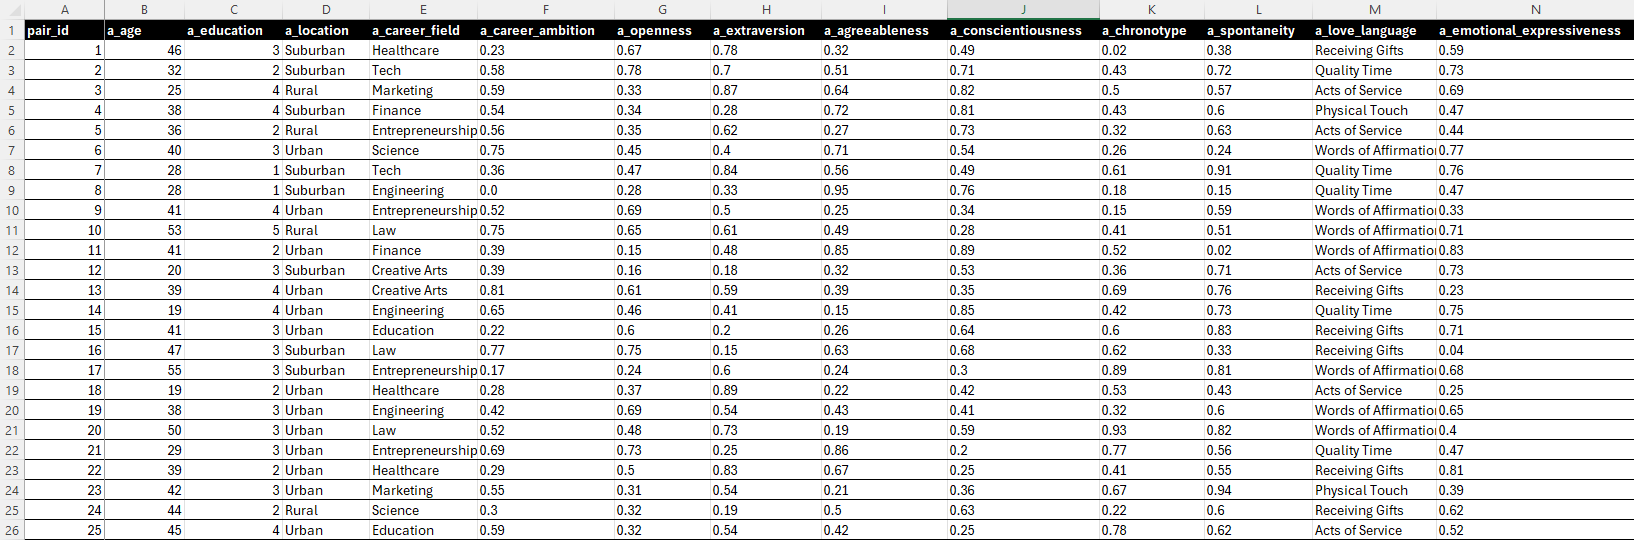
\includegraphics[width=0.95\textwidth]{Pictures/24_records_a.png}
  \caption{Extracto de los datos del Individuo A correspondientes a los 24 primeros emparejamientos evaluados. Se aprecian las variables demográficas y las métricas del modelo \textit{Big Five}.}
  \label{fig:registros_a}
\end{figure}

\begin{figure}[H]
  \centering
  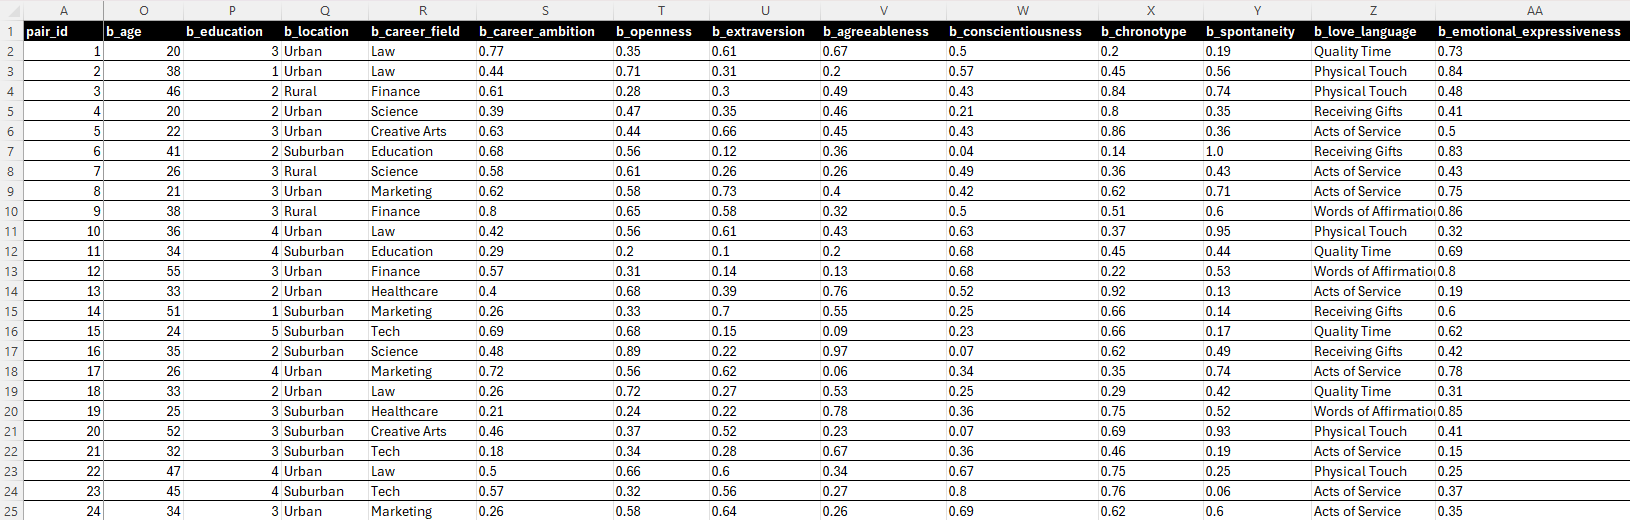
\includegraphics[width=0.95\textwidth]{Pictures/24_records_b.png}
  \caption{Extracto de los datos del Individuo B correspondientes a los 24 primeros emparejamientos. Nótese la obligatoria correspondencia del campo \texttt{pair\_id} con el Individuo A para posibilitar el emparejamiento.}
  \label{fig:registros_b}
\end{figure}

Más allá de las características predictoras de cada usuario individual, el sistema evalúa el resultado de la diada mediante sus variables objetivo. Siguiendo con la muestra de los 24 primeros registros analizados, la Figura~\ref{fig:ejemplo_targets} expone visualmente los campos \texttt{compatibility\_score}, \texttt{compatible} y \texttt{relationship\_longevity\_months} para estas interacciones. En su conjunto, estas tres métricas son las encargadas de definir empíricamente qué tan ``satisfactoria'' ha resultado la relación, constituyendo la verdad terreno sobre la cual el algoritmo optimizará sus predicciones.

\begin{figure}[H]
  \centering
  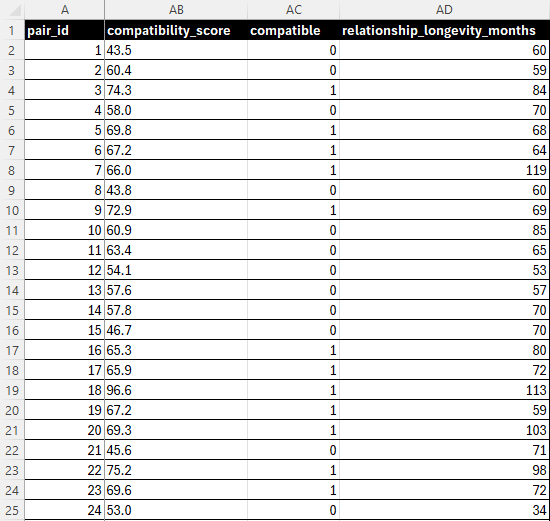
\includegraphics[width=0.50\textwidth]{Pictures/24_records_comp.png}
  \caption{Representación de las variables objetivo que definen el nivel de satisfaction y viabilidad de la relación, correspondientes a los 24 primeros registros del conjunto de datos.}
  \label{fig:ejemplo_targets}
\end{figure}


\section{Análisis de los datos y Detección de Sesgos}
\label{sec:analisis_datos}
El Análisis Exploratorio de Datos (EDA) se ha enfocado en modelar las dinámicas de interacción intra-pareja, identificar patrones predictivos viables y detectar posibles sesgos (estadísticos o estructurales) en el conjunto de datos. Para ello se ejecutó un estudio sistemático apoyado en herramientas de visualización de datos avanzadas.

\subsection{Análisis de Sesgos: Variables Objetivo (Score, Clases y Longevidad)}
En esta primera serie de visualizaciones evaluamos el comportamiento y las distribuciones de nuestras tres variables objetivo (\textit{targets}) principales (ver Figura \ref{fig:distribuciones_targets}):

\begin{itemize}
    \item \textbf{Densidad del Score de Compatibilidad:} El primer gráfico revela que la puntuación base se ajusta a una distribución aproximadamente normal. No observamos polarizaciones extremas (sesgos hacia los extremos 0 o 100), lo que nos indica una distribución sana y equilibrada para utilizarla como métrica de regresión.
    \item \textbf{Balance de Clases (Éxito Relacional):} El gráfico central muestra un ligero desbalance natural en la etiqueta binaria \texttt{compatible}, con casi un 43\% de casos de éxito frente a un 57\% de fracasos. Al ser un desbalance moderado y altamente representativo de las dinámicas relacionales del mundo real, podemos prescindir de aplicar técnicas artificiales de sobremuestreo (como SMOTE) para nuestros modelos iniciales.
    \item \textbf{Distribución de Longevidad:} El histograma de la derecha revela cómo se distribuye el tiempo de vida de las relaciones en meses. Se observa una alta concentración de frecuencias en los primeros meses (rupturas tempranas típicas), disminuyendo gradualmente conforme avanza el tiempo. Nuestro modelo de regresión tendrá que aprender a interpretar esta asimetría temporal natural.
\end{itemize}

\begin{figure}[H]
  \centering
  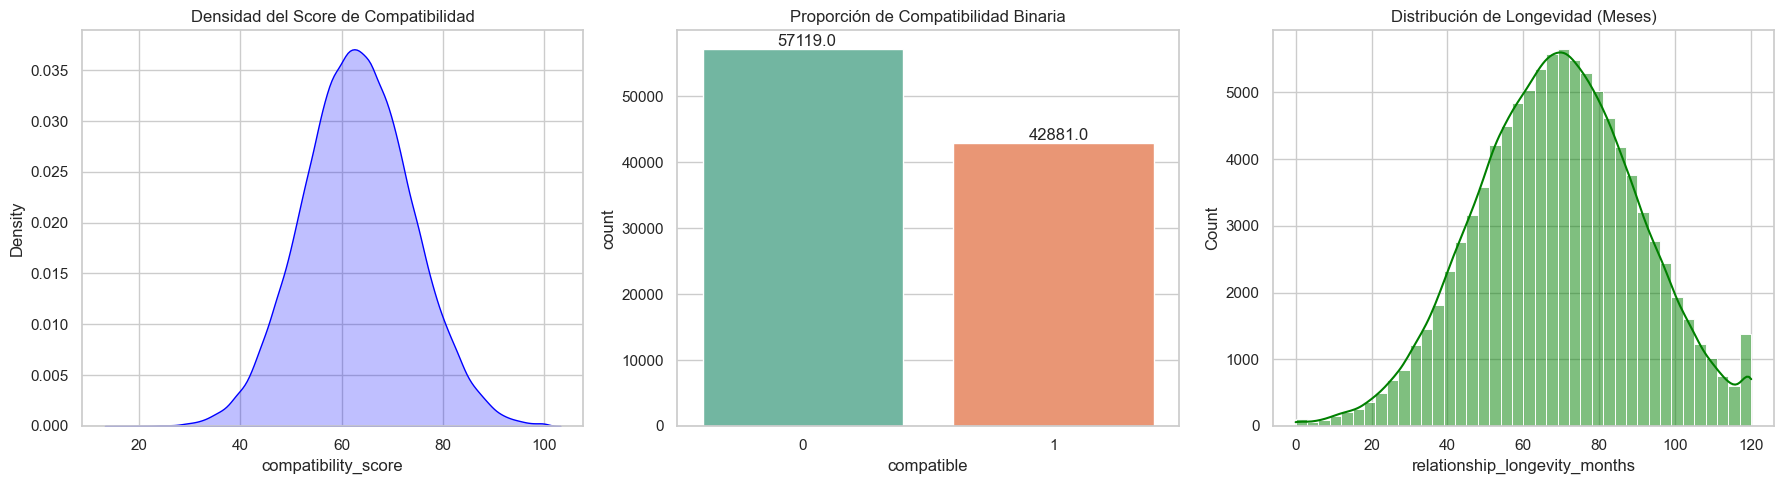
\includegraphics[width=0.95\textwidth]{Pictures/distribuciones_targets.png} 
  \caption{Distribución de las variables objetivo: densidad del score (izq.), balance de clases (centro) y longevidad (der.).}
  \label{fig:distribuciones_targets}
\end{figure}

Para ahondar en esta distribución temporal, se procedió a agrupar los registros de longevidad en bloques de 5 meses. La Figura~\ref{fig:sesgo_supervivencia_5meses} ilustra claramente el \textbf{Sesgo de Supervivencia} inherente al problema. Existe una concentración masiva de rupturas (incompatibilidades, en rojo) en las primeras etapas. Esta visualización confirma que la predicción de longevidad será un reto algorítmico donde el modelo deberá aprender a discriminar qué factores otorgan resiliencia a largo plazo frente a los fracasos tempranos.

\begin{figure}[H]
  \centering
  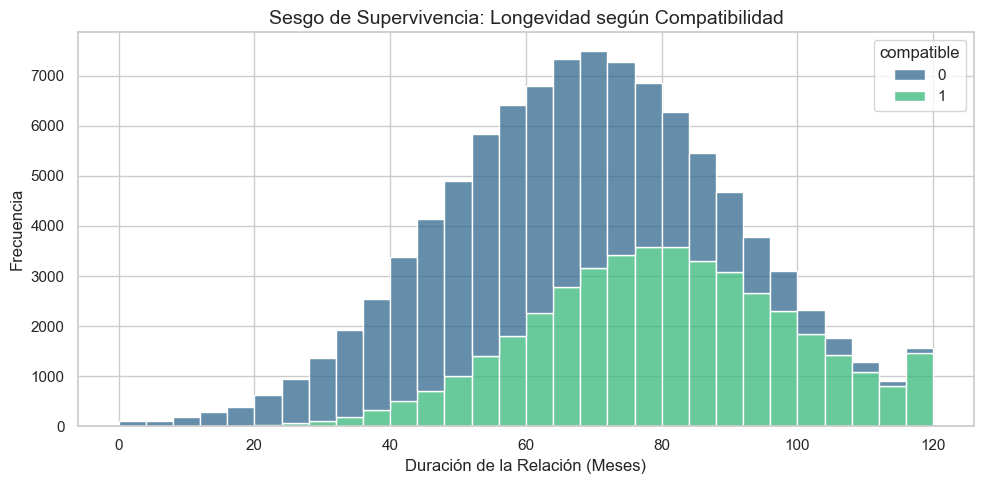
\includegraphics[width=0.85\textwidth]{Pictures/sesgo_supervivencia_5meses.png} 
  \caption{Distribución de registros según su longevidad agrupada en intervalos de 5 meses. Se aprecia la fuerte caída temprana de las relaciones incompatibles.}
  \label{fig:sesgo_supervivencia_5meses}
\end{figure}


\subsection{Análisis de Sesgos Estructurales: Ambición y Brecha de Edad}
Estas visualizaciones exponen cómo las diferencias relativas o "brechas" absolutas afectan al éxito de la pareja, revelando patrones estructurales clave (ver Figura \ref{fig:sesgos_estructurales}):

\begin{itemize}
    \item \textbf{Afinidad en Ambición:} El gráfico de densidad KDE confirma que las parejas compatibles (representadas en azul) tienden a agruparse fuertemente cerca de la línea de identidad diagonal, lo que significa que poseen niveles de ambición profesional equiparables. Por el contrario, las parejas incompatibles (en rojo) presentan una mayor dispersión.
    \item \textbf{Diferencia de Edad (\textit{Age Gap}):} El diagrama de violín nos muestra la distribución de la brecha de edad entre parejas exitosas y fallidas. Podemos observar cómo la forma de las distribuciones varía ligeramente, revelando que el algoritmo deberá aprender a sopesar esta diferencia absoluta como un posible factor de penalización relacional.
\end{itemize}

\begin{figure}[H]
  \centering
  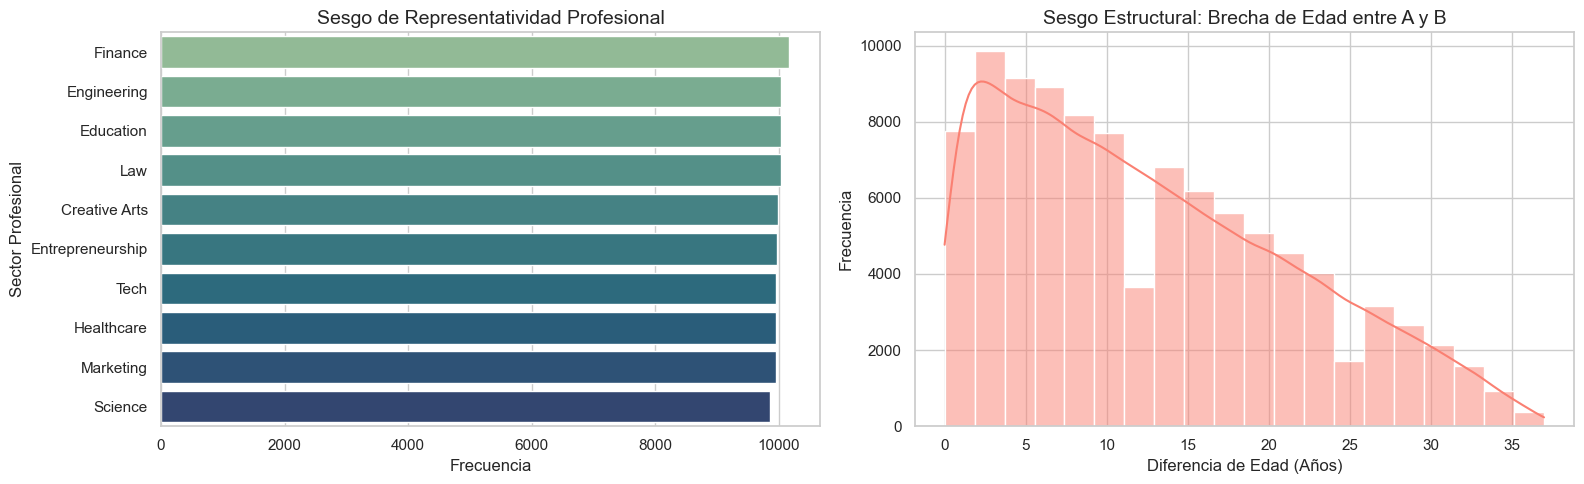
\includegraphics[width=0.95\textwidth]{Pictures/sesgos_estructurales.png} 
  \caption{Análisis de sesgos estructurales: Afinidad en ambición profesional (izquierda) y diagrama de violín para la diferencia de edad (derecha).}
  \label{fig:sesgos_estructurales}
\end{figure}


\subsection{Análisis de Sesgos de Interacción: Lenguajes del Amor}
Esta visualización es crítica para entender cómo interactúan las variables categóricas entre ambos individuos. La Figura~\ref{fig:matriz_lenguajes_amor} muestra la matriz de contingencia térmica cruzando los lenguajes del amor.

\begin{itemize}
    \item \textbf{Tasa de Compatibilidad por Cruce:} Este mapa de calor (\textit{heatmap}) demuestra visualmente el principio sociológico de \textit{homofilia}. Las celdas que conforman la diagonal principal (donde ambos individuos comparten exactamente el mismo lenguaje del amor) presentan tasas de éxito porcentual significativamente más altas. Esto nos indica de forma clara que el algoritmo deberá nutrirse de variables de interacción construidas mediante \textit{Feature Engineering} para captar estas coincidencias.
\end{itemize}

\begin{figure}[H]
  \centering
  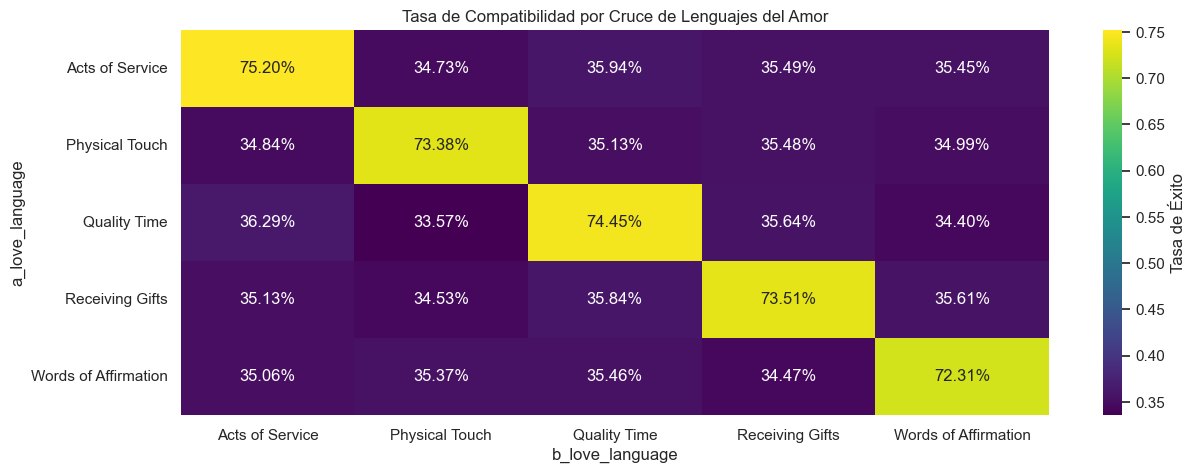
\includegraphics[width=0.75\textwidth]{Pictures/matriz_lenguajes_amor.png}
  \caption{Matriz de contingencia térmica (\textit{Heatmap}): Tasa de compatibilidad porcentual según el cruce de los lenguajes del amor entre ambos individuos.}
  \label{fig:matriz_lenguajes_amor}
\end{figure}

\subsection{Ingeniería de Características (\textit{Feature Engineering})}
Con el fin de trasladar estas relaciones geométricas, mitigar sesgos de representación y proporcionar un marco matemático viable para los algoritmos de \textit{Machine Learning}, se ejecutó un proceso profundo de Ingeniería de Características:

\begin{enumerate}
    \item \textbf{Distancia Euclidiana de Personalidad:} Se procedió a calcular la norma euclidiana vectorial entre el conjunto de rasgos psicológicos (\textit{Big Five} y expresividad emocional) de ambos individuos. Esta transformación matemática consolida múltiples variables en un predictor continuo robusto que penaliza las divergencias extremas de carácter.
    \item \textbf{Disimilitud Continua:} Se derivaron nuevas métricas calculando las diferencias absolutas (brechas) en atributos numéricos clave, tales como la edad, la ambición profesional y el cronotipo.
    \item \textbf{Interacciones Categóricas (Efecto Espejo):} Las coincidencias en variables nominales fueron codificadas como indicadores booleanos. El estudio determinó que presentar coincidencias exactas en estas variables incrementa notablemente la probabilidad de éxito. Por ejemplo, compartir el mismo campo profesional (\texttt{match\_career} = 1) eleva la tasa de compatibilidad promedio hasta el 53.7\%.
\end{enumerate}

Las características derivadas se han consolidado en la Tabla~\ref{tab:diccionario_pesos}, clasificadas en función de si su impacto resulta positivo o negativo para el algoritmo predictivo.

\begin{table}[H]
\centering
\begin{tabular}{llp{8.5cm}}
\hline
\textbf{Característica (Feature)} & \textbf{Impacto} & \textbf{Descripción y Justificación Técnica} \\ \hline
\texttt{match\_career} & Positivo (+) & Coincidencia exacta en el sector profesional. Correlaciona positivamente con el éxito relacional. \\
\texttt{match\_love\_language} & Positivo (+) & Compartir el lenguaje del amor favorece la complementariedad y entendimiento afectivo. \\
\texttt{personality\_distance} & Negativo (-) & Distancia euclidiana en el \textit{Big Five}. A mayor distancia geométrica, disminuye la probabilidad de éxito. \\
\texttt{diff\_career\_ambition} & Negativo (-) & Brecha absoluta en ambición profesional. Las asimetrías severas actúan como factor fuertemente disruptivo. \\ \hline
\end{tabular}
\caption{Diccionario de variables interactivas: características con pesos positivos y negativos}
\label{tab:diccionario_pesos}
\end{table}

Para asegurar una integración óptima en la futura arquitectura de software y prevenir la transferencia indebida de información (\textit{Data Leakage}), estas transformaciones se orquestaron a través de la clase \texttt{ColumnTransformer} (perteneciente a la librería \textit{scikit-learn}). Este \textit{pipeline} aplica una estandarización a las variables continuas y una codificación \textit{One-Hot} a las categóricas, dejando el conjunto preparado para la etapa de inferencia y modelado.

\section{Evaluación del rendimiento y Métricas}
\label{sec:evaluacion_metricas}
En el marco de la integración del algoritmo \textit{Cupid} dentro de una arquitectura software real, hemos definido tres métricas operativas principales para evaluar el rendimiento del sistema, diseñadas específicamente para reflejar la experiencia relacional de los usuarios. Las métricas establecidas son:

\begin{itemize}
    \item Dada una pareja, predecir si son compatibles o no, utilizando la métrica de compatibilidad.
    \item Dada una pareja, predecir si son compatibles y estimar su tiempo de duración (longevidad).
    \item Dada una persona, predecir qué otra persona es la más compatible con ella.
\end{itemize}

A continuación, se formaliza matemáticamente cada uno de estos enfoques:

\subsection{1. Predicción de Compatibilidad Binaria}
Para determinar si dos individuos son compatibles, el sistema genera primero una métrica de compatibilidad continua. Sea $u_A$ y $u_B$ los vectores de características de la Persona A y la Persona B. Definimos la función de compatibilidad del modelo como $S(u_A, u_B) \in [0, 100]$.

La predicción binaria final $\hat{y}$ (compatible o no compatible) se formaliza aplicando un umbral de decisión $\tau$ (típicamente establecido en 65, según la distribución empírica del dataset):

\begin{equation}
    \hat{y}_{A,B} = 
    \begin{cases} 
      1 & \text{si } S(u_A, u_B) \ge \tau \\
      0 & \text{si } S(u_A, u_B) < \tau
    \end{cases}
\end{equation}

El rendimiento de esta predicción binaria sobre el conjunto de validación se evalúa mediante la Exactitud (\textit{Accuracy}) y el \textit{F1-Score}, contrastando $\hat{y}_{A,B}$ con el éxito real de la pareja, donde el \textit{score} continuo $S$ actúa como el motor discriminador.

\subsection{2. Estimación de Longevidad Relacional}
De forma complementaria a la clasificación de la compatibilidad, el sistema debe ser capaz de estimar la duración temporal de la relación. Definimos la función de estimación de longevidad como $L(u_A, u_B)$, la cual proyecta el tiempo en meses.

La evaluación conjunta asume que la longevidad es un problema de regresión. Para cuantificar la precisión matemática de nuestra estimación respecto a la longevidad real $Y_{A,B}$, se define la función de pérdida mediante el Error Cuadrático Medio (RMSE), penalizando de forma severa las discrepancias extremas en la predicción del tiempo de duración:

\begin{equation}
    RMSE = \sqrt{\frac{1}{N} \sum_{i=1}^{N} \Big(Y_{A_i,B_i} - L(u_{A_i}, u_{B_i})\Big)^2}
\end{equation}

Donde $N$ representa el total de parejas evaluadas. Esta métrica permite comprender el error de la estimación en la misma escala temporal (meses) de la variable objetivo.

\subsection{3. Recomendación (Matching óptimo)}
El objetivo de mayor impacto en el producto no evalúa parejas de forma aislada. En su lugar, dada una persona específica $u_A$ y un conjunto de candidatos disponibles $C = \{c_1, c_2, \dots, c_m\}$, el algoritmo debe \textbf{predecir qué persona es la más compatible}, presentando un \textit{ranking} ordenado en orden descendente según $S(u_A, c_j)$. 

Para evaluar la calidad de este emparejamiento múltiple, se adoptan métricas del estado del arte de los Sistemas de Recomendación:

\begin{itemize}
    \item \textbf{Mean Reciprocal Rank (MRR):} Cuantifica la rapidez del sistema para ofrecer el emparejamiento óptimo en la interfaz, localizando la posición (o rango) de la \textit{primera} persona verdaderamente compatible recomendada a $u_A$.
    
    \begin{equation}
        MRR = \frac{1}{|U|} \sum_{i=1}^{|U|} \frac{1}{rank_i}
    \end{equation}
    
    Donde $|U|$ es el número total de usuarios consultados, y $rank_i$ representa la posición en la lista del primer candidato compatible. Su maximización asegura que el usuario no tendrá que hacer \textit{scroll} para encontrar a su mejor prospecto.

    \item \textbf{Mean Average Precision (MAP):} Complementando al MRR, el MAP evalúa la calidad global del ranking, calculando la Precisión Media (\textit{AP}) para el top $K$ de personas más compatibles recomendadas:

    \begin{equation}
        MAP = \frac{1}{|U|} \sum_{u=1}^{|U|} \left( \frac{1}{m_u} \sum_{k=1}^{K} P_u(k) \cdot rel_u(k) \right)
    \end{equation}

    Donde $m_u$ es el número de posibles parejas exitosas para $u$; $K$ es el límite de recomendaciones visualizadas; $P_u(k)$ es la precisión hasta la posición $k$; y $rel_u(k)$ es 1 si el candidato en la posición $k$ resulta compatible, y 0 en caso contrario. 
\end{itemize}

El planteamiento conjunto de estas tres dimensiones garantiza que la optimización algorítmica responda con exactitud matemática a las necesidades funcionales del producto y la experiencia del usuario.
